%%%%%%%%%%%%%%%%%%%%%%%%%%%%%%%%%%%%%%%%%
% Propuesta de Desarrollo
% LaTeX Template
% Version 1.0 (06/02/2014)
%
% Original authors:
% Belén Beltran (belubeltran@gmail.com)
% Pablo Ariel Rodriguez (prodriguez@fi.uba.ar)
% Federico Rossi (federicomrossi@gmail.com)
%
%%%%%%%%%%%%%%%%%%%%%%%%%%%%%%%%%%%%%%%%%



%------------------------------------------------------------------------------
%	PACKAGES AND OTHER DOCUMENT CONFIGURATIONS
%------------------------------------------------------------------------------

\documentclass{book}

% Paquetes generales
\usepackage[left=4cm, right=3cm, top=4cm, bottom=3cm, paperwidth=210mm, paperheight=297mm, headsep=1.5cm]{geometry}
\usepackage[utf8]{inputenc}
\usepackage[svgnames]{xcolor} % Required to specify font color
\usepackage{gensymb}

% Paquetes para estilos
\usepackage{textcomp}
\usepackage{setspace}
\usepackage{colortbl}
\usepackage{color}
\usepackage{color}
\usepackage{upquote}
\usepackage{xcolor}
\usepackage{listings}
\usepackage{caption}
\usepackage[T1]{fontenc}
\usepackage[scaled]{beramono}

% Paquetes extras
\usepackage{amssymb}
\usepackage{float}
\usepackage{graphicx}
\usepackage[export]{adjustbox}
\usepackage{url}
\usepackage[toc,page]{appendix}

% Paquete Matematica
\usepackage{mathtools}

% Paquetes para header y footer
\usepackage{fancyhdr}



% Definición de preferencias para la impresión de código fuente.
%% Colores
\definecolor{gray99}{gray}{.99}
\definecolor{gray95}{gray}{.95}
\definecolor{gray85}{gray}{.85}
\definecolor{gray75}{gray}{.75}
\definecolor{gray50}{gray}{.50}



\usepackage{titlesec}

% \titleformat*{\section}{\LARGE\bfseries}
% \titleformat*{\subsection}{\Large\bfseries}
% \titleformat*{\subsubsection}{\large\bfseries}
% \titleformat*{\paragraph}{\large\bfseries}
% \titleformat*{\subparagraph}{\large\bfseries}

% Ocultamos numeración de las secciones
%%\setcounter{secnumdepth}{0}




%------------------------------------------------------------------------------
%	TITLE PAGE
%------------------------------------------------------------------------------

\newcommand*{\titleGM}{\begingroup % Create the command for including the title page in the document
\newcommand*{\sepline}{\color{gray85}\rule[0.5ex]{30em}{0.55pt}}
	
	
\begin{center}

	\vspace*{1.5cm} 

	
\includegraphics[width=9cm]{images/graferator-logo.png} \\[12\baselineskip]

	
	\colorbox{gray95}{
		\parbox[t]{1.0\linewidth}{
			% \centering \fontsize{50pt}{80pt}\selectfont % The first argument for fontsize is the font size of the text and the second is the line spacing - you may need to play with these for your particular title
			\vspace*{0.7cm} % Space between the start of the title and the top of the grey box
			
			\centering {\Huge\bfseries\color{gray50}\fontfamily{fvs}\selectfont Carpeta de Desarrollo}\par % Tagline or further description	
			
			\vspace*{0.7cm} % Space between the end of the title and the bottom of the grey box
		}
	}\\[10\baselineskip]


	% \sepline \\[1\baselineskip]
		\Large Belén Beltran \\
		\large \textit{belubeltran@gmail.com} \\ \medskip
		\Large Pablo Ariel Rodriguez \\
		\large \textit{prodriguez@fi.uba.ar} \\ \medskip
		\Large Federico Martin Rossi \\ 
		\large \textit{federicomrossi@gmail.com} \\

		\bigskip\bigskip\bigskip\bigskip

		\large 2do. Cuatrimestre 2014 \\ \smallskip
		\large 75.52 Taller de Programación II \\ \smallskip
		\large Facultad de Ingeniería, Universidad de Buenos Aires \\ \smallskip

\end{center}

	% }}
\endgroup}

\renewcommand{\chaptername}{Capítulo}
\renewcommand{\contentsname}{Contenido}
% \titleformat{\chapter}[display]
%   {\normalfont\bfseries\huge\color{black}}
%   {\chaptertitlename\ \thechapter}{0.5em}{\textbf\Huge} 
% \titleformat{\section}
%   {\normalfont\Large\fontfamily{fvs}\bfseries\color{black}}
%   {\thesection}{1em}{\Large}
% \titleformat{\subsection}
%   {\normalfont\Large\fontfamily{fvs}\color{cyan}}
%   {\thesection}{1em}{\Large}

% \titleformat{\chapter}[hang] 
% {\normalfont\Huge\fontfamily{fvs}}{\chaptertitlename\ \thechapter:}{0.5em}{\Huge} 
% \titleformat{\section}{\normalfont\Large\fontfamily{fvs}}{\thesection}{1em}{\Large}


%% FIGURAS
\captionsetup[figure]{labelfont=bf,textfont=it}
%% TABLAS
\captionsetup[table]{labelfont=bf,textfont=it}

% COMANDOS

%% Titulo de las cajas de código
\renewcommand{\lstlistingname}{Código}
%% Titulo de las figuras
\renewcommand{\figurename}{Imagen}
%% Titulo de las tablas
\renewcommand{\tablename}{Tabla}
%% Referencia a los códigos
\newcommand{\refcode}[1]{\textit{Código \ref{#1}}}
%% Referencia a las imagenes
\newcommand{\refimage}[1]{\textit{Imagen \ref{#1}}}




%------------------------------------------------------------------------------
%	HEADER AND FOOTER
%------------------------------------------------------------------------------


% \pagestyle{fancy}



%------------------------------------------------------------------------------
%	BLANK DOCUMENT
%------------------------------------------------------------------------------

\begin{document}

\pagenumbering{roman}
% \setcounter{page}{0}

% \pagestyle{empty} % Removes page numbers
\thispagestyle{empty}


% This command includes the title page
\titleGM
% \thispagestyle{empty}
% \newpage \textit{}
% \thispagestyle{empty}
% \newpage \textit{}
% \thispagestyle{empty}



%
% TEXTOS PREVIOS
%
\section*{\bfseries\color{black}Antes de empezar}

Esta guía asume que el lector se encuentra familiarizado con el sistema operativo \textit{Microsoft Windows} (versión XP y posteriores) y aquellos basados en GNU/Linux. Es decir, se considera que el usuario se encuentra mínimamente en condiciones de desenvolverse en el entorno en el cual se ejecuta la aplicación, razón por la cual no se explican temas como la utilización de cuadros de diálogo, asistentes o el exploradores de carpetas.
\bigskip


\section*{Objetivo}

El objetivo principal de esta guía es ayudar y guiar al usuario en la instalación, así como también en la utilización de \textbf{Graferator} haciendo hincapié en las características y opciones más relevantes que se presentan en este. 
\bigskip


\section*{\bfseries\color{black}Cómo leer esta guía}

Se recomienda al usuario leer esta guía teniendo a la vista de su pantalla el software ejecutándose. Esto le permitirá poder realizar los pasos aquí detallados a medida que avanza en la lectura, logrando asimilar más fácilmente la disposición de las distintas opciones mencionadas y la forma en que estas deben ser utilizadas.
\bigskip


\section*{\bfseries\color{black}Organización}

La guía está compuesta de capítulos que agrupan las distintas funcionalidades provistas por la aplicación y que se encuentran relacionadas entre sí. Las secciónes que conforman los capítulos detallan los pasos a seguir para poder hacer uso de dichas funcionalidades.



% ÍNDICE
\tableofcontents
\newpage
\thispagestyle{empty}
\pagenumbering{arabic}
\thispagestyle{empty}
\thispagestyle{empty}



%
% CAPITULO 1
%
\chapter{Introducción}


% CAPITULO 1
% Descripción general
\section{Descripción general}
	
	El presente documento se centra en el desarrollo de \textit{Graferator}, una aplicación de computadora cuyo objetivo es llevar a cabo el estudio de la teoría de grafos con el fin de ser utilizado en la enseñanza y el aprendizaje de la respectiva temática.
	\par
	Recordando que un grafo es un conjunto conformado por vértices o nodos unidos por enlaces conocidos como aristas o arcos, el software permitirá de manera gráfica la confección y manipulación de estos a través de una interfaz de usuario intuitiva y simple.
	\par
	Los usuarios podrán hacer uso de dos modalidades de ejecución, a saber:
	\medskip

	\begin{itemize}
		\renewcommand{\labelitemi}{\scriptsize\tiny$\blacksquare$} 
		\itemsep=10pt \topsep=0pt \partopsep=0pt \parskip=0pt \parsep=10pt
		
		\item \textbf{Modo aprendizaje}: resolución paso a paso con avance a solicitud del aprendiz (al siguiente paso o al resultado final).

		\item \textbf{Modo autoevaluación}: resolución paso a paso con elaboración guiada del resultado de cada paso a cargo del aprendiz. Confirmación de la corrección del resultado con opción de reintentar en caso de que fuere incorrecto, o ver el resultado correcto.

	\end{itemize}
	\medskip



% CAPITULO 1
% Funcionalidad
\section{Funcionalidad}

	Graferactor constará de las funcionalidades básicas que se requieren para el armado de un grafo. Inicialmente se le permitirá al usuario la creación de un \textit{Grafo Orientado} o un \textit{Grafo No Orientado}. 
	\par
	Además, para cada una de estas opciones se deberá elegir si se desea comenzar a partir de un grafo vacío o si se prefiere generar un grafo aleatorio, especificando la cantidad de vértices y aristas a tomar en cuenta.
	\par
	De esta manera, la aplicación permitirá:
	\medskip

	\begin{itemize}
		\renewcommand{\labelitemi}{\scriptsize\tiny$\blacksquare$} 
		\itemsep=2pt \topsep=0pt \partopsep=0pt \parskip=0pt \parsep=0pt
		
		\item el alta o baja de vértices,

		\item el alta o baja de aristas o arcos,

		\item el borrado del grafo,

		\item la ponderación de arcos.

	\end{itemize}
	\medskip


% CAPITULO 1
% Algoritmos
\section{Algoritmos}

	Una vez armado el grafo deseado, Graferator permitirá a los usuarios aplicar sobre este una serie de algoritmos que ayudarán y aportarán al estudio de sus propiedades.
	\par
	Como se ha adelantado previamente, cada algoritmo podrá ser ejecutado en dos modos distintos (modo aprendizaje y modo autoevaluación). Así, los usuarios no solamente comprenderán el grafo, sino que también adquirirán conocimientos acerca de cómo funcionan los algoritmos aplicables a estos.
	\par
	De esta manera, habiendo confeccionado el grafo, se podrán efectuar los siguientes algoritmos:


	\begin{itemize}
		\renewcommand{\labelitemi}{\scriptsize\tiny$\blacksquare$} 
		\itemsep=2pt \topsep=0pt \partopsep=0pt \parskip=0pt \parsep=0pt
		
		\item Recorrido en profundidad,

		\item Recorrido en anchura,

		\item Prueba de aciclidad.

	\end{itemize}
	\medskip

	\noindent Si el grafo es orientado, además será posible ejecutar los siguientes:
	\medskip

	\begin{itemize}
		\renewcommand{\labelitemi}{\scriptsize\tiny$\blacksquare$} 
		\itemsep=2pt \topsep=0pt \partopsep=0pt \parskip=0pt \parsep=0pt
		
		\item Recorrido topológico en anchura y en profundidad (si es acícilico),

		\item Obtención de la cerradura transitiva,

		\item Obtención de componentes fuertemente conexas.

	\end{itemize}
	\medskip

	\noindent Si se trata de un grafo orientado con aristas ponderadas:
	\medskip

	\begin{itemize}
		\renewcommand{\labelitemi}{\scriptsize\tiny$\blacksquare$} 
		\itemsep=2pt \topsep=0pt \partopsep=0pt \parskip=0pt \parsep=0pt
		
		\item Algoritmo de caminos mínimos de Dijkstra con un mismo origen (requiriéndose que todas las ponderaciones no sean negativas),

		\item Algoritmo de caminos mínimos de Floyd entre todos los pares de nodos,

		\item Algoritmo de flujos máximos de Ford-Fulkerson.

	\end{itemize}
	\medskip

	\noindent Por último, si el grafo es no orientado:
	\medskip

	\begin{itemize}
		\renewcommand{\labelitemi}{\scriptsize\tiny$\blacksquare$} 
		\itemsep=2pt \topsep=0pt \partopsep=0pt \parskip=0pt \parsep=0pt
		
		\item Algoritmo de árbol de expansión de coste mínimo.

	\end{itemize}
	\medskip



% CAPITULO 1
% Ejecución de algoritmos
\section{Ejecución de algoritmos}

	Dispuesto el grafo sobre la zona de diseño y elegido el algoritmo junto con el modo en el cual se ejecutará el mismo, el usuario deberá dar comienzo a la simulación. Para esto la interfaz contará con una serie de controles con los cuales se indicará el inicio o el fin de la ejecución, así como también controles con los que se podrá desplazar a lo largo de esta.
	\par
	A medida que se corre el algoritmo se podrá visualizar paso a paso la ejecución de este sobre el grafo mediante colores que facilitarán la comprensión del avance en el mismo.
	\par
	En el momento en que se realiza la elección del algoritmo, habrá una ventana interna en la que se visualizará el pseudocódigo respectivo. En la ejecución se resaltarán una a una las líneas de las sentencias de manera tal que los usuarios realicen un seguimiento detallado de todo el proceso, siendo esto de complemento y apoyo en el aprendizaje del funcionamiento de los distintos algoritmos. A esto se le incluye el conteo del número de sentencias ejecutadas. De esta manera los usuarios tendrán la información necesaria para realizar distintas tareas de análisis, tales como el cálculo de la complejidad algorítmica, refactorización de los algoritmos, entre otros.
	\par
	Cada paso podrá ser deshecho dado que no solo existirán controles para realizar el avance, sino también para llevar a cabo el retroceso en cualquier instancia del proceso.



%
% CAPITULO 2
%
\chapter{Herramientas de Desarrollo}


% CAPITULO 2
% Lenguaje y entorno de programación
\section{Lenguaje y entorno de programación}


\subsection{Lenguaje Java}


\subsection{WindowBuilder (GUI)}


\subsection{Eclipse IDE}


\subsection{Maven}




% CAPITULO 2
% Controlador de versiones
\section{Controlador de versiones}

\subsection{Git}

\subsection{GitHub}



% CAPITULO 2
% Herramientas para documentación
\section{Herramientas para documentación}


\subsection{LaTeX}


\subsection{Draw.io}




%
% CAPITULO 3
%
\chapter{Diseño de la solución}


% CAPITULO 3
% Estructura general
\section{Arquitectura}

	En el primer capítulo de este documento hemos detallado la funcionalidad con la que contara Graferator. Allí hemos podido ver que será necesaria una interfaz gráfica la cual será la mediadora entre el usuario y la aplicación. 
	\par
	Para contar con un entorno visual va a ser necesario que exista un motor o modelo que lo respalde. Esto es, un módulo que se encarge de manejar aquellos aspectos abstractos e internos que permitirán que el software funcione correctamente. Dado esto es que se cree conveniente utilizar como base en el desarrollo de la aplicación el \textit{patrón de arquitectura Model-View-Controller} o mayormente conocido por sus siglas MVC.
	\bigskip

% Imagen 
\begin{figure}[H]
	\centering
	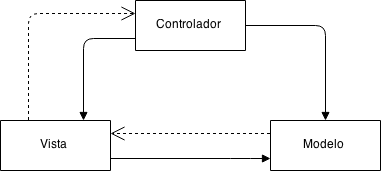
\includegraphics[width=0.6\textwidth]{images/01-MVC.png}
	\medskip
	\caption{Diagrama del patrón de arquitectura MVC}
	\medskip
\end{figure}
	\bigskip
	
	El patrón MVC hará posible separar los datos y la lógica de negocio de la interfaz de usuario (también conocida por las siglas GUI) y el módulo encargado de gestionar los eventos y las comunicaciones. Para esto, dicho patrón propone la construcción de tres módulos descentralizados: \textit{Modelo}, \textit{Vista} y \textit{Controlador}. De esta manera, se establecen por un lado los componentes que hacen a la representación de la información y por otro lado se constituyen componentes para la interacción con el usuario. En la \textit{Imagen 3.1} se muestra un diagrama representativo de este patrón.
	\par
	La totalidad de la aplicación será desarrollada en base a dicha arquitectura en gran medida por los grandes beneficios que significan poseer el modelo y la lógica separados de todo lo restante. Por esta razón, en los siguientes apartados se profundizará sobre cada módulo y se describirán los componentes que lo conforman como así también la forma en la que trabajan entre sí y se comunican con el exterior para lograr los objetivos planteados por el alcance del software.
	\newpage


% CAPITULO 3
% Modelo
\section{Modelo}

	Como ya se ha adelantado, el \textit{Modelo} es la representación de la información con la cual nuestro sistema operará. Por lo tanto, gestionará todos los accesos a los datos, tanto consultas como actualizaciones. Mediante solicitudes de la \textit{Vista}, este módulo le enviará la información requerida para ser mostrada y visualizada por el usuario. Estas peticiones llegarán al modelo a través del módulo \textit{Controlador}.
	\bigskip


\subsection{Componentes básicos}

	Primeramente, encontraremos que el modelo necesitará representar a los constituyentes básicos de los grafos. En la \textit{Imagen 3.2} se puede observar un primer diagrama de clases UML en donde se encuentran las clases \textit{Vertice} y \textit{Arista}. Ambas implementarán a la interfaz \textit{Selectable}, quien simplemente establece que tanto los objetos Arista como Vertice son seleccionables. A su vez, Arista hereda de clase que define a objetos con peso, de manera tal que las aristas podrán ser ponderadas cuando así lo requieran.
	\par
	Por otro lado, la clase Vertice también implementa las interfaces \textit{Serializable} y \textit{Comparable}, las cuales le dan caracteristicas para poder ser serializados y poder ser comparados respectivamente.
	\bigskip\bigskip


% Imagen 
\begin{figure}[H]
	\centering
	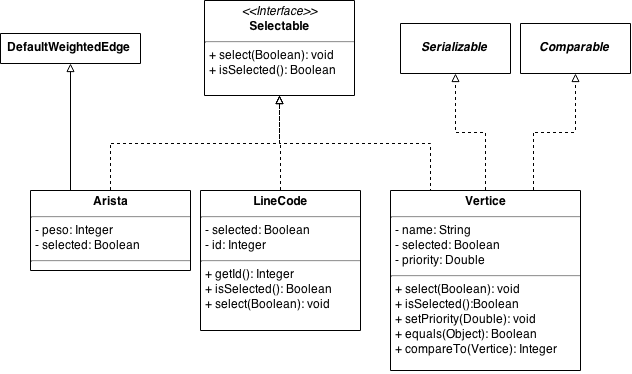
\includegraphics[width=1\textwidth]{images/01-01.png}
	\medskip
	\caption{texto \\ texto}
	\medskip
\end{figure}
\medskip



\subsection{Representación del Grafo}

	Conformadas las componentes básicas, necesitamos una entidad que modele al grafo. Esta clase la denominaremos \textit{GraphModel}. Esta hará uso de un conjunto de objetos Vertice relacionados entre sí por objetos Arista. En la \textit{Imagen 3.3} se puede observar el diagrama de clases en donde se muestra como está conformado GraphModel.



% Imagen 
\begin{figure}[H]
	\centering
	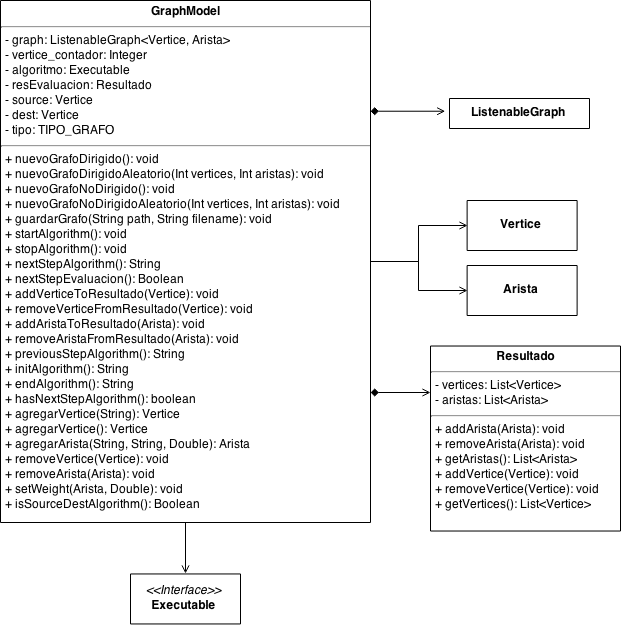
\includegraphics[width=0.8\textwidth]{images/01-03.png}
	\medskip
	\caption{texto \\ texto}
	\medskip
\end{figure}
\bigskip


\subsection{Representación de los Algoritmos}


% Imagen 
\begin{figure}[H]
	\centering
	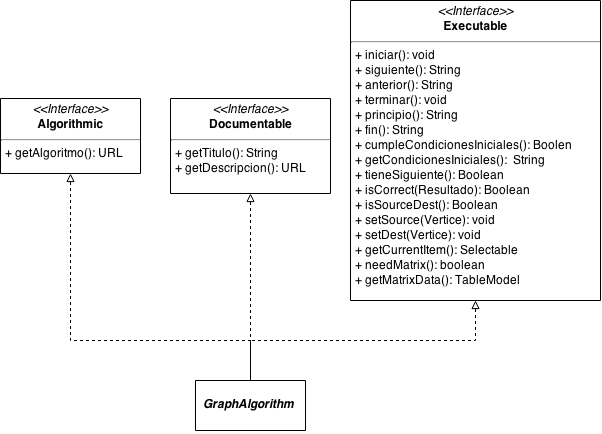
\includegraphics[width=0.8\textwidth]{images/01-02.png}
	\medskip
	\caption{texto \\ texto}
	\medskip
\end{figure}
\bigskip




% Imagen 
\begin{figure}[H]
	\centering
	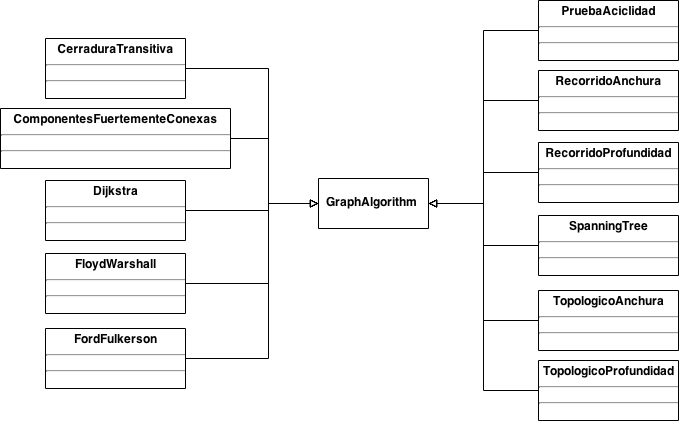
\includegraphics[width=0.8\textwidth]{images/01-04.png}
	\medskip
	\caption{texto \\ texto}
	\medskip
\end{figure}
\bigskip



% CAPITULO 3
% Vista
\section{Vista}


% Imagen 
\begin{figure}[H]
	\centering
	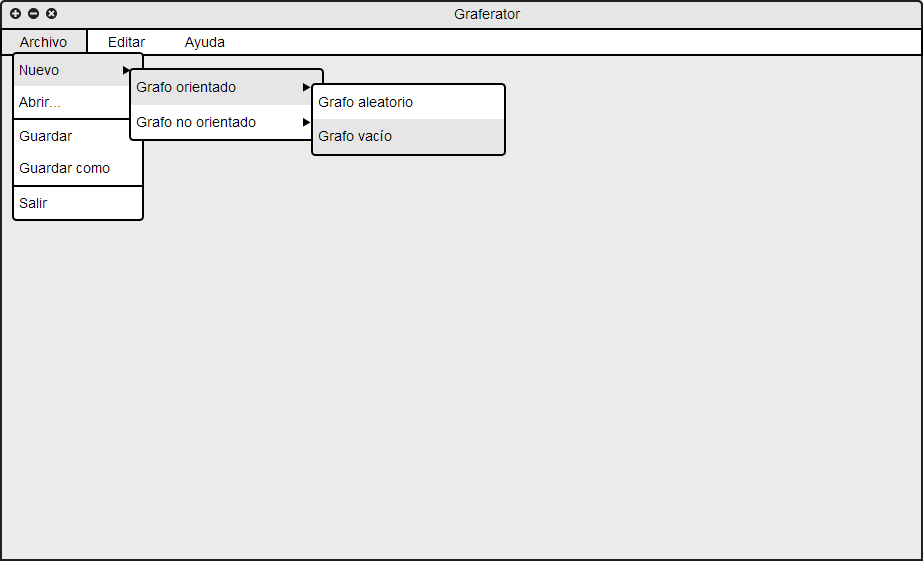
\includegraphics[width=0.9\textwidth]{images/02-01.png}
	\medskip
	\caption{texto \\ texto}
	\medskip
\end{figure}
\bigskip


% Imagen 
\begin{figure}[H]
	\centering
	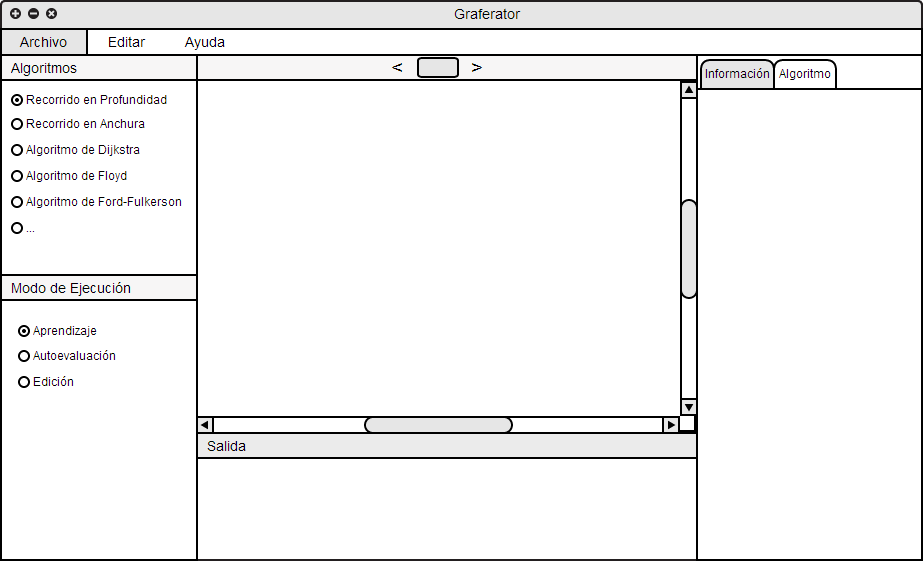
\includegraphics[width=0.9\textwidth]{images/02-02.png}
	\medskip
	\caption{texto \\ texto}
	\medskip
\end{figure}
\bigskip


% Imagen 
\begin{figure}[H]
	\centering
	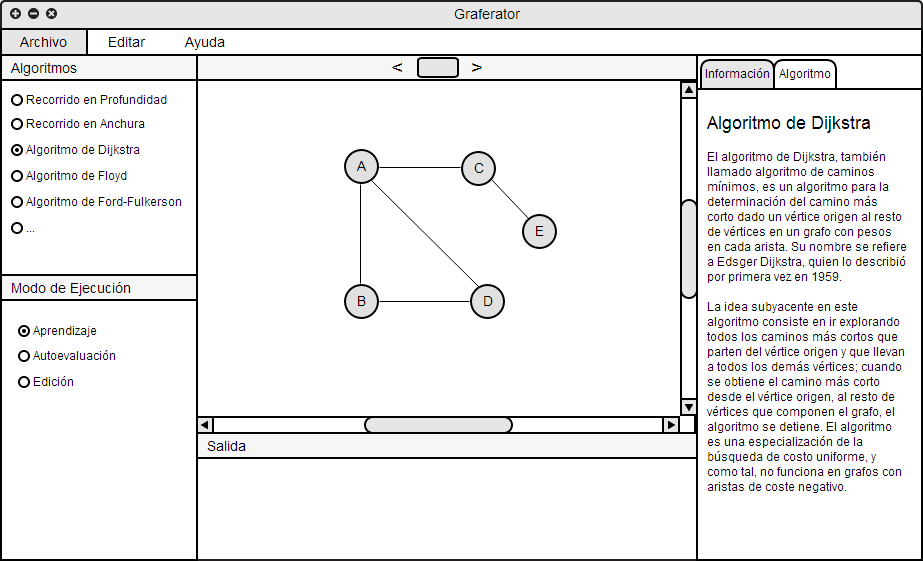
\includegraphics[width=0.9\textwidth]{images/02-03.png}
	\medskip
	\caption{texto \\ texto}
	\medskip
\end{figure}
\bigskip



% CAPITULO 3
% Controlador
\section{Controlador}



















% CAPITULO 3
% []
% \section{[]}




%
% CAPITULO 4
%
\chapter{Distribución de tareas}


% CAPITULO 4
% []
% \section{[]}




\end{document}